\section{Auswertung}
\label{sec:Auswertung}


Im folgenden werden die Theoriewerte aus \autoref{tab:literatur}, die der Literatur entnommen wurden, verwendet \cite{x_ray_database}.
Die zugehörigen Winkel jeweiliger Materialien wurden dann nach \autoref{eq:tbd} berechnet.
Es folgt 
\begin{equation*}
  \theta = \arcsin \left( \frac{h c}{2 d E} \right)
\end{equation*}
Dabei wurde $n = 1$ gesetzt und $\lambda$ durch die bekannte Gleichung 
\begin{equation*}
  \lambda = \frac{h \cdot c}{E}
\end{equation*}
berechnet.
Weiterhin werden für die Theoriewerte der Kupferlinien
\begin{align*}
  E_{\mathrm{K}, \mathrm{abs}} &=8,987 \mathrm{keV} \, \\
  E_{\mathrm{K}, \alpha}^{\mathrm{lit}} &=8,048 \mathrm{keV} 
\end{align*}
und
\begin{equation*}
  E_{\mathrm{K}, \beta}^{\mathrm{lit}} =8,906 \mathrm{keV} \, .
\end{equation*}
angenommen \cite{x_ray_database}.
Daraus resultieren dann auch durch \autoref{tbd}, \autoref{tbd} und \autoref{tbd} die $\sigma_i$'s
\begin{align*}
  \sigma_{1} &=3,29 \, ,\\
  \sigma_{2} &=12,38 \\ 
  \intertext{und}
  \sigma_{3} &=21,68 \, .
\end{align*}

%  Anhang ?
 
\begin{table}
  \centering
  \caption{Theoriewerte für die Messwerte \cite{x_ray_database}.}
  \label{tab:literatur}
  \begin{tabular}{ccccc} 
    \hline Element & $Z$ & $\sigma_{\mathrm{K, Lit}}$& $E_{\mathrm{K, Lit}}$ in keV & $\theta_{\mathrm{K, Lit}}$ in \\
    \hline $\mathrm{Zn}$ & 30 & 3,57 & 9,65 & 18,60  \\
    $\mathrm{Ga}$ & 31 & 3,60 & 10,38 & 17,25  \\
    $\mathrm{Ge}$ & 32 & 3,66 & 11,11 & 16,08  \\
    $\mathrm{Br}$ & 35 & 3,84 & 13,48 & 13,20  \\
    $\mathrm{Rb}$ & 37 & 3,94 & 15,2 & 11,68   \\
    $\mathrm{Sr}$ & 38 & 3,98 & 16,12 & 11,01  \\
    $\mathrm{Zr}$ & 40 & 4,09 & 18,0 & 9,85    \\
    \hline
  \end{tabular}
\end{table}

\subsection{Überprüfung der Bragg - Bedingung}
Zunächst soll die Bragg-Bedingung nachgewiesen werden.
Die Messwerte sind in \autoref{fig:bragg} aufgetragen.
Der Sollwinkel liegt bei $28°$.
Mittels Python wurde das Maximum bei tbd gefunden. %%%%%%%%%%%%%%%%%%%%%%%%%%%%%%%%%%%%%%%%%%%%%%%%%%%%%%%%%

% \begin{figure}
%   \centering
%   \caption{Messwerte zur Untersuchung der Bragg-Bedingung}
%   \label{fig:bragg}
%   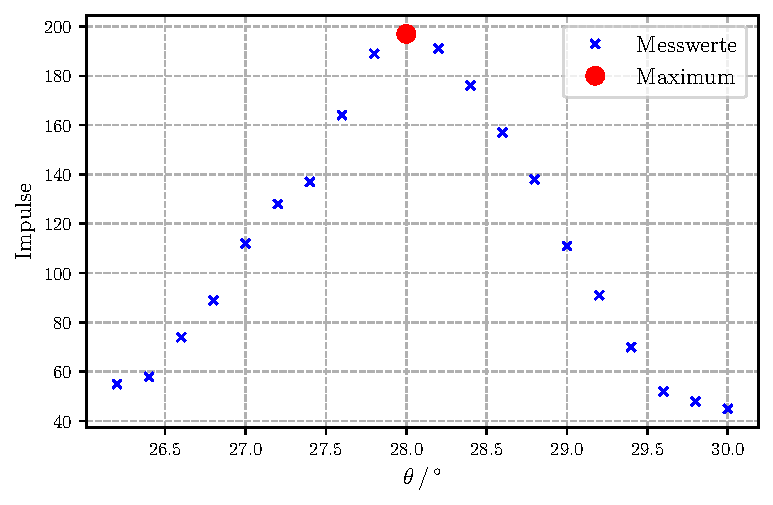
\includegraphics[width=0.5 \linewidth]{build/bragg.pdf}
% \end{figure}

\subsection{Emissionsspektrum von Kupfer}
Im folgenden wird das Emissionsspektrum von Kupfer untersucht.
Aufgetragen sind die Messdaten, die über einen USB-Stick beim Versuch gespeichert und ausgelesen wurden, in \autoref{fig:kupfer1}.
Das Maximum der Bremsstrahlung lässt sich ungefähr bei $tbd °$ einordnen.
Um die charakteristische Strahlung genauer zu untersuchen werden nur Messwerte zwischen tbd und tbd in \autoref{fig:kupfer2} abgebildet.
Aus den Peaks lassen sich dann die Energien mit \autoref{eq:tbd} zu
\begin{align*}
  E_{\text{K}_\alpha} = tbd \\ % \qty{tbd}{keV}\\
  \intertext{und} \\
  E_{\text{K}_\beta} = tbd % \qty{tbd}{keV}
\end{align*}
berechnet.
Die Halbwertsbreiten liefern die Energiedifferenzen
\begin{align*}
  \increment E_{\text{K}_\alpha} &= tbd \\ % \qty{tbd}{keV}\\
  \intertext{und}
  \increment E_{\text{K}_\beta} &= tbd % \qty{tbd}{keV} \, .
\end{align*}
Für das Auflösungsvermögen gilt die Gleichung
\begin{equation*}
  A = \frac{E}{\increment E} \, ,
\end{equation*}
woraus die Werte
\begin{align*}
  A_{\text{K}_\alpha} = tbd\\
  \intertext{und} \\
  A_{\text{K}_\beta} = tbd
\end{align*}
bestimmt werden.
Schließlich werden noch die Abschirmkonstanten mit \autoref{tbd}, \autoref{tbd} und \autoref{tbd} bestimmt.
Hier wird für das errechnen von $\sigma_2$ und $\sigma_3$ der theoretische Wert von $\sigma_1$ herangezogen, da sonst keine Bestimmung der anderen Möglich wäre. 
Es folgt
\begin{align*}
  \sigma_{1} &= 3,29 \, ,\\
  \sigma_{2} &= tbd \\ 
  \intertext{und}
  \sigma_{3} &= tbd \, .
\end{align*}

% \begin{figure}
%   \centering
%   \caption{Messreihe zur Untersuchung des Emissionsspektrums von Kupfer.}
%   \label{fig:kupfer1}
%   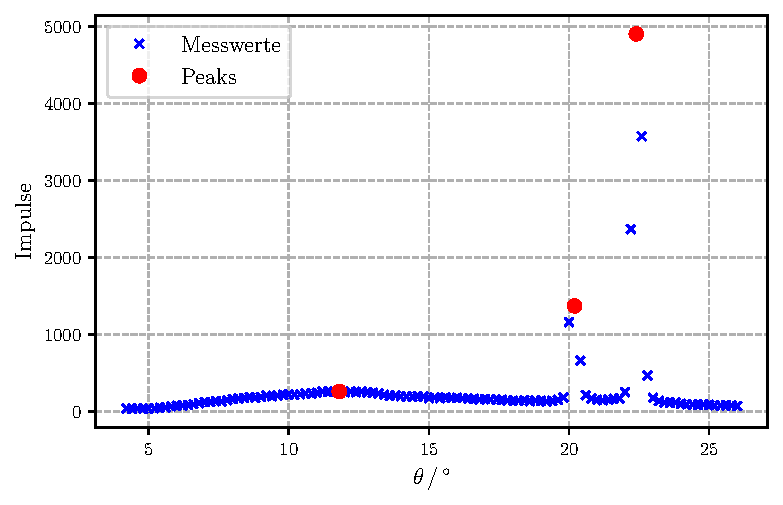
\includegraphics[width=0.5 \linewidth]{build/kupfer1.pdf}
% \end{figure}

% \begin{figure}
%   \centering
%   \caption{Reduzierte Messreihe zur Untersuchung des Emissionsspektrums von Kupfer.}
%   \label{fig:kupfer1}
%   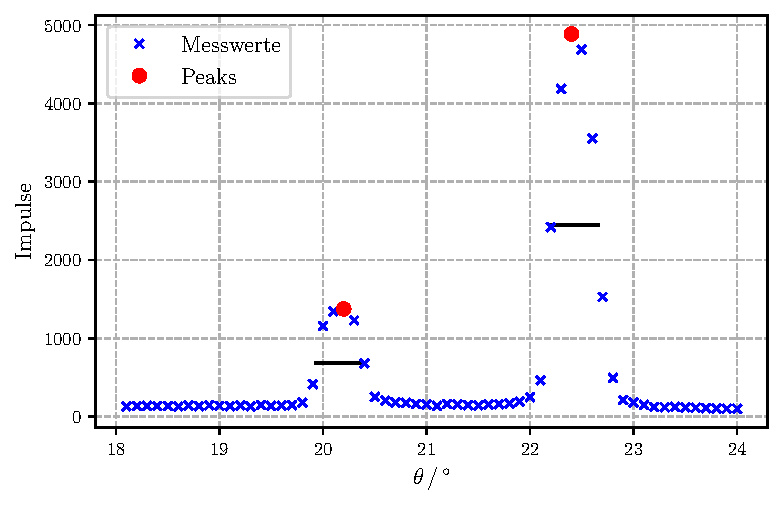
\includegraphics[width=0.5 \linewidth]{build/kupfer2.pdf}
% \end{figure}

\subsection{Analyse der Absorptionsspektren}

Abschließend sollen die Absorptionsspektren verschiedenster Materialien ermittelt werden.
Hierfür wird die Zählrate $N$ der gemessenen Impulse gegen den Winkel $\theta$ aufgetragen.
Die Absorptionskante wird in den folgenden Plots eingezeichnet.
Zusätzlich wird eine vertikale Linie durch die Mitte dieser Kante gelegt.
Die Mitte ist durch die Gleichung
\begin{equation*}
  I_K = \frac{I_K^\text{min} + I_K^\text{max}}{2}
\end{equation*}
festgelegt. Dabei beschreiben $I_K^\text{min}$ und $I_K^\text{max}$ das Intensitätsminimum /- maximum der Absorptionskante.
Daraus lässt sich dann der Winkel $\theta$ bestimmen, woraus Schließlich die Energie sowie die Abschirmkonstante bestimmt werden kann.

\subsubsection{Zink}
% \begin{figure}
%   \centering
%   \caption{Absorptionsspektrum von Zink.}
%   \label{fig:zink}
%   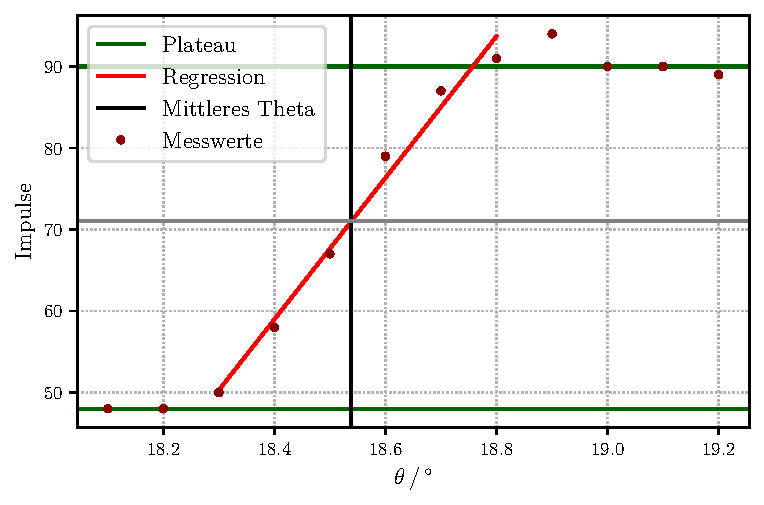
\includegraphics[width=0.5 \linewidth]{build/zink.pdf}
% \end{figure}

\subsubsection{Gallium}
% \begin{figure}
%   \centering
%   \caption{Absorbtionsspektrum von Gallium.}
%   \label{fig:gallium}
%   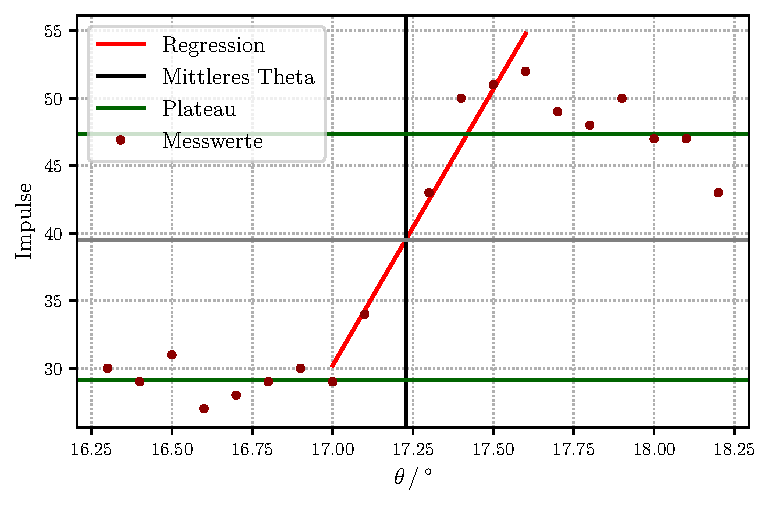
\includegraphics[width=0.5 \linewidth]{build/gallium.pdf}
% \end{figure}

\subsubsection{Brom}
% \begin{figure}
%   \centering
%   \caption{Absorbtionsspektrum von Brom.}
%   \label{fig:brom}
%   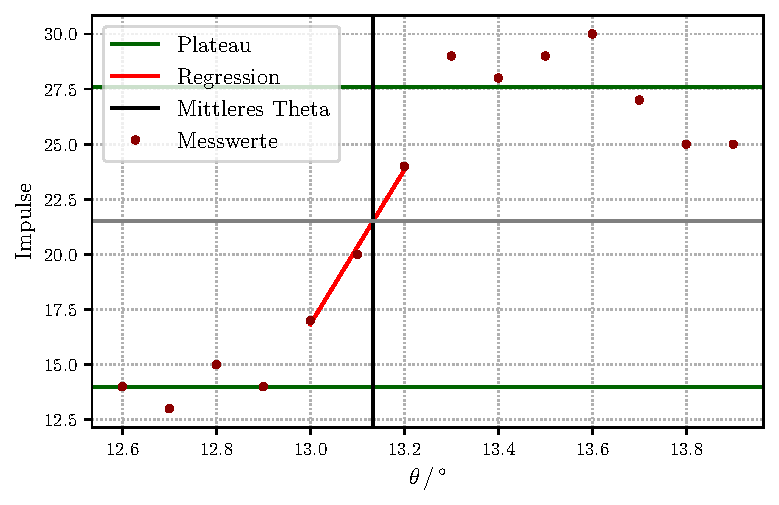
\includegraphics[width=0.5 \linewidth]{build/brom.pdf}
% \end{figure}

\subsubsection{Rubidium}
% \begin{figure}
%   \centering
%   \caption{Absorbtionsspektrum von Rubidium.}
%   \label{fig:rubidium}
%   \includegraphics[width=0.5 \linewidth]{build/rubidium.pdf}
% \end{figure}

\subsubsection{Strontium}
% \begin{figure}
%   \centering
%   \caption{Absorbtionsspektrum von Strontium.}
%   \label{fig:strontium}
%   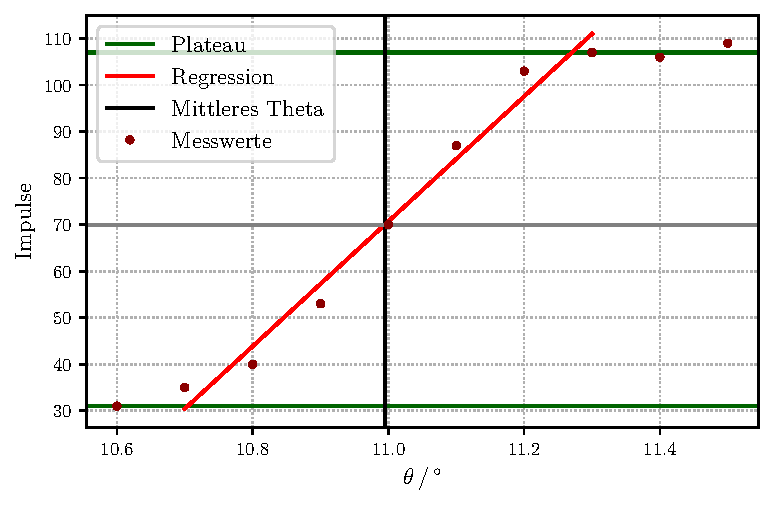
\includegraphics[width=0.5 \linewidth]{build/strontium.pdf}
% \end{figure}

\subsubsection{Zirkonium}
% \begin{figure}
%   \centering
%   \caption{Absorbtionsspektrum von Zirkonium.}
%   \label{fig:zirkonium}
%   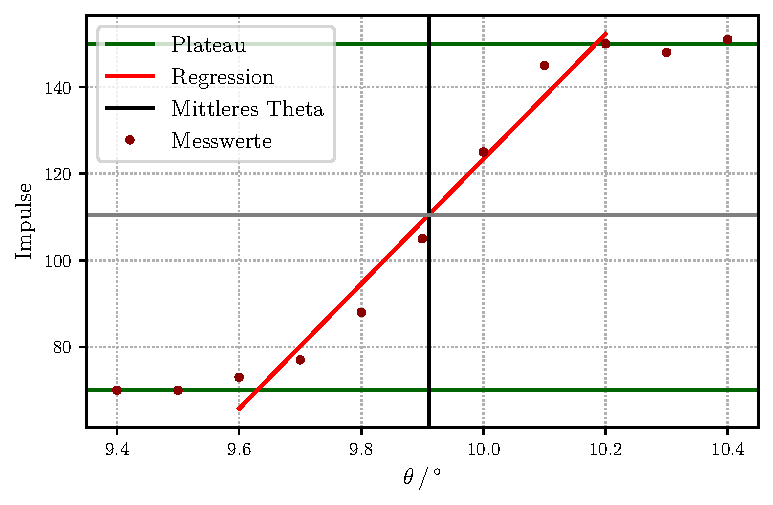
\includegraphics[width=0.5 \linewidth]{build/zirkonium.pdf}
% \end{figure}

\subsection{Moseley's Gesetz}
Nun wird mit den gewonnenen Energien das Moseley'sche Gesetz verifiziert werden.
Hierfür wird der Ansatz
\begin{equation*}
  f(Z) = m \cdot Z + b
\end{equation*}
gewählt. Dabei werden die Wurzeln der ermittelten Energien gegen die zugehörigen $Z$'s aufgetragen.
Die Regression ist dargestellt in \autoref{fig:moseley}.
Aus der linearen Regression mittels Python ergeben sich die Parameter
\begin{align*}
  m = \qty{1}{\eV}^{-\frac{1}{2}} && \text{und} && b  = \qty{1}{\eV}^{-\frac{1}{2}} \, .
\end{align*}
Daraus lässt sich nun die experimentell ermittelte Rydberg-Energie zu
\begin{equation*}
  E_\text{Ryd} = \frac{1}{m^2} = tbd
\end{equation*}
berechnen.

% \begin{figure}
%   \centering
%   \caption{Regressionsgerade zur Verifizierung des Moseley'schen Gesetzes.}
%   \label{fig:moseley}
%   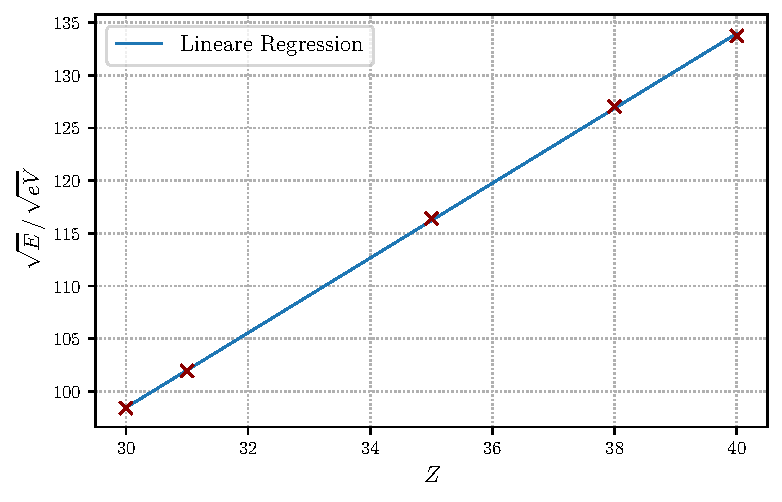
\includegraphics[width=0.5 \linewidth]{build/moseley.pdf}
% \end{figure}